%
% introduction
\section{Interface}
\label{sec:raspberry-software}
As anticipated, the software run on the Raspberry Pi is made following the
paradigm of object-oriented programming. Made in C++/Qt making extensive use
of the proprietary classes of the framework and the Standard Template Library
(STL). This program has some dependencies with regard to the thermal camera
drivers supplied by the manufacturer and are 32-bit, since the Raspberry Pi 3,
described in \ref{sec:raspi3}, is equipped with a 32-bit ARM Cortex-A53
processor. These allow total control of the camera. The second dependency is the
Raspicam library which allows the interface with the RGB camera allowing the
image acquisition.
%
\begin{figure}[htb]
	\centering
	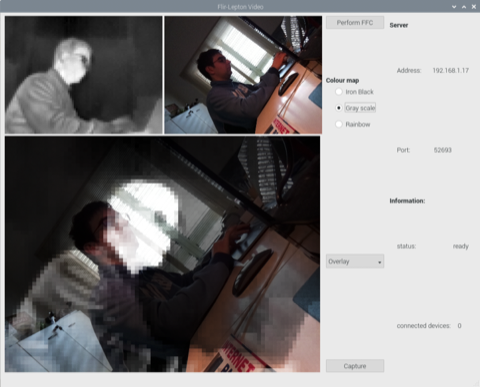
\includegraphics[width=0.65\textwidth]{grayscale.png}
	\caption{User interface run on Raspberry Pi 3b.}
	\label{fig:software-main-ui}
\end{figure}
%
% interface
Continuing a user interface has been created through the use of widgets, this is
divided into three areas. The first area shows the video streams acquired
separately in two labels, the third larger label shows the two streams mixed
through filters made available as default the overlay filter is used. It was
preferred not to perform a match of the images with pixel-by-pixel recalculation
for two reasons: the first due to the high difference in size of the sensors as
that of the thermal camera is $80 \times 60$ pixels while the Raspicam is $3280
\times 2464$ pixels. Furthermore motivation is due to not aggravate the 
computational load on the CPU.
The second area provides some controls for the user, in fact it is
possible to save thermal images on files during the acquisition. you can change
the heat map applied to the image on the fly by choosing from three different
possibilities, in the figure you can observe the result. 
Finally, it is possible to modify the mixing filter, also on the fly, of the
video streams to obtain different effects to improve visibility or to increase
details.
The last section of the user interface shows the information relating
to the TCP socket used for sending the video stream to other devices.
%
% image ui
\begin{figure}[htb]
    \centering
    \subfloat[][\emph{lava}.\label{subfig:lava-map}]
        {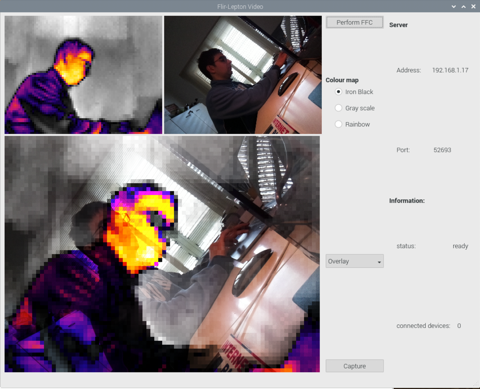
\includegraphics[width=.30\textwidth]{lava.png}} \quad
    \subfloat[][\emph{grayscale}.\label{subfig:grayscale-map}]
        {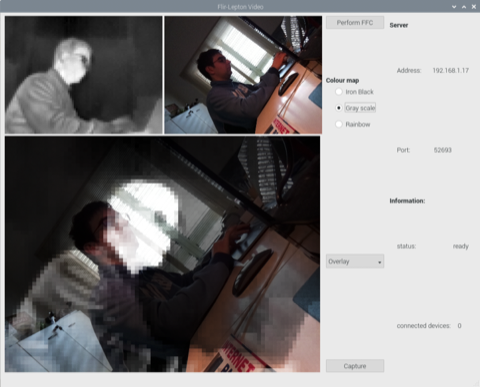
\includegraphics[width=.30\textwidth]{grayscale.png}} \quad
    \subfloat[][\emph{rainbow}.\label{subfig:rainbow-map}]
        {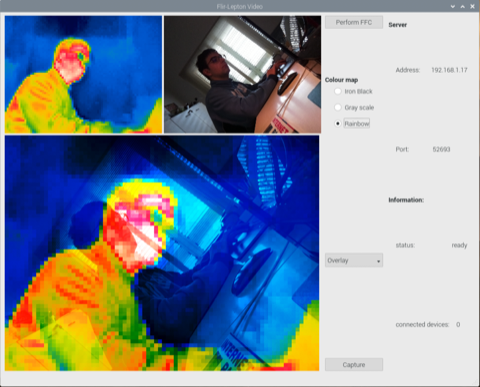
\includegraphics[width=.30\textwidth]{rainbow.png}}
    \caption{Result colourization applied to thermal camera data.}
    \label{fig:reuslt-maps}
\end{figure}
%
% software analysis 
\subsection{Software Analysis}
\label{ssec:raspberry-softw-analysis}
The user interface is run on the main thread, in order to maximize the
performance of the executed code the image acquisition operation is performed in
the secondary thread. Thanks to the use of the signal and slot system of Qt, 
introduced before in (\ref{ref:soft-signal-slot}), it is possible to update the 
labels without blocks typical of multi-threaded programming. 
The difficulty of concurrent programming usually consists in
synchronizing the access to resources by different threads that act in
competition on the same resources. Having two or more threads accessing the same
data simultaneously can lead to unexpected and unwanted results. 
In fact, without the application of particular programming techniques, it is not
possible to predict in a deterministic way, at the time of execution, when that
specific thread will be executed: their progression depends on the priorities
decided by the scheduler of the operating system and not by the programmer. 
In fact, multiple threads can access the same variable and modify its content or
value. Therefore, synchronization techniques such as mutual exclusion are used
to solve the problem. As a result, ideally a thread should execute code as
independent of the rest of the program as possible. Furthermore, errors in
synchronization between threads are often very difficult to detect because their
occurrence essentially depends on the environment in which the program is run.
The synchronization of one thread with another is normally necessary to allow
them to communicate with each other and to return the results of a function to
the main process; it is normally done through \emph{mutex}\cite{wiki:thread}.
Analysing the code of the thread that takes care of acquiring the images we can 
see that it proceeds without mutex\footnote{The mutex class is a synchronization
primitive that can be used to protect shared data from being simultaneously
accessed by multiple threads.}, but uses the signal and slot system as mentioned
before.
%
% code list
\inputminted[frame=lines,framesep=2mm, linenos=true, autogobble, breaklines=true, fontsize=\scriptsize, firstline=36, lastline=100]{c++}{software/code/leptonthread.cpp} 
\captionof{listing}{Infinite loop thread cameras.\label{lst:rasp-leptonthread}}
%
\pagebreak
Going to analyse in detail the infinite loop, reported in the
listing (\ref{lst:rasp-leptonthread}), executed in a thread other than the main
one that manages only the main interface, it can be observed that:
\begin{itemize}
\item (line 37--56) When the function starts, an instance of the \texttt{QImage}
type object is instantiated to contain the image acquired during the cycle. The
parameters of the frame size are provided and the color space this allows to
increase the speed of the cycle as it will not be cyclically cancelled and
reallocated the same, but will be reused. The communication with the thermal
camera is opened via the SPI port if the cycle is not started or if the
communication is interrupted the communication is closed.
% code list
%\begin{minipage}{\linewidth}
%\centering
%\inputminted[bgcolor=bg,frame=lines,framesep=2mm, linenos=true, autogobble, breaklines=true, fontsize=\scriptsize, firstline=36, lastline=61]{c++}{software/code/leptonthread.cpp} 
%\captionof{listing}{Data acquisition from SPI.}
%\label{lst:rasp-leptonthread-data} 
%\end{minipage}
%
\item (line 66--78) The main cycle is to acquire data from the saved camera
registers, as the order is MSB\footnote{MSB can also stand for "most significant
byte". \emph{Big-endian processor}: When data is loaded into a multi-byte
register, the first byte (with the lowest address) is the most significant byte
of the data.\cite{56322}}, reversed in according to LSB\footnote{LSB can also
stand for "least significant byte". \emph{Little-endian processor}: When data is
loaded into a multi-byte register, the first byte (with the lowest address) is
the least significant byte of the data.\cite{56322}}. The values are then scaled
to obtain a consistent representation of the hot and cold areas. Then the color
map is applied to color the raw data obtained from the scaling process described
above.
%% code list
%\begin{minipage}{\linewidth}
%\centering 
%\inputminted[bgcolor=bg,frame=lines,framesep=2mm, linenos=true, autogobble, breaklines=true, fontsize=\scriptsize, firstline=79, lastline=108]{c++}{software/code/leptonthread.cpp} 
%\captionof{listing}{Flip the MSB and LSB and colouration.} 
%\label{lst:rasp-leptonthread-MSB-LSB} 
%\end{minipage}\linebreak
%%
\item (line 79--97) Finally, signals are output for the coloured thermal image,
for the RGB image acquired by the Raspicam library and passed through the slot
and the last resulting from mixing of previous two depend on effect of selected
in UI interface.
%% code list
%\begin{minipage}{\linewidth}
%\centering 
%\inputminted[bgcolor=bg,frame=lines,framesep=2mm, linenos=true, autogobble, breaklines=true, fontsize=\scriptsize, firstline=36, lastline=117]{c++}{software/code/leptonthread.cpp} 
%\captionof{listing}{Infinite loop thread cameras.} 
%\label{lst:rasp-leptonthread} 
%\end{minipage}
\end{itemize}
As can be seen, the cycle proceeds without mutuals or blocking conditions, in
fact, as previously described, it is possible to change the color map or the
mixing tool on the fly.
%
% analysing comunication
% description socket tcp
\newpage
\section{Communication systems}
\label{sec:software-TCPSocket}
In digital data communications, wiring together two or more devices is one of
the first steps in establishing a network. As well as this hardware requirement,
software must also be addressed. The Open System Interconnection (OSI) model
proposed by the International Organization for Standardization (ISO) is a
standard way to structure communication software that is applicable to any
network. The model has been standardized by ISO and International
Telecommunication Union (ITU) Telecommunication Standardization Sector (ITU-T)
which is the organization coordinating standards for telecommunications. 
The
communication is based on low-level message passing between the communicating
systems.
\begin{itemize}
\item A wants to communicate with B; 
\item A builds a message addressing B; 
\item A executes a call to the communication module to send the message to B.
\end{itemize}
Of course, A and B need to speak the same language, i.e., they need to agree on the meaning
of the bits being sent. The protocols define the rules for communication. 
When
data is exchanged through a computer network, the system rules are called a
network protocol. A protocol must define the syntax, semantics, and timing of
communication (i.e. how, what and when); the specified behaviour is typically
independent of how it is to be implemented. Syntax: refers to the structure or
the format of the data. Semantics: the way in which the bit patterns are
interpreted. Timing: specify when the data can be sent and how fast it will be.
Another term is synchronization.
The communication between two nodes of a network occurs by sending messages. a
message is broken down into a sequence of packets, and each packet is
transmitted individually.
The structure includes some control bits at the beginning of the message called
\emph{header} and at the end called \emph{footer}.
the control bits can contain information such as: the sending node of the
packet, the recipient node of the package, package length information,
information that allows you to verify the correctness of the package. \cite{mandrioli2008informatica}
%
\subsection{Architecture}
\label{ssec:soft-client-server}
Client/server architectures are based on the functional division of IT
applications into two categories. Few computers act as servers, run a particular
program that allows the computer to receive requests and send replies.
As shows in figure (\ref{fig:client-server architecture}).\hfill \break
The clients, on the other hand, run a program that allows them to send requests and
receive replies. Client/server applications are two-level architectures, that
is, the first level is the client and the second level is the server. The
interaction protocols between client and server are quite simple. among the
advantages of client/server architectures we have the simplicity of
construction and the possibility of having easy-to-use clients.\\ 
Disadvantages include the risk of overloading the computer acting as a server 
and the communication channel with which the server is connected to the network.\cite{mandrioli2008informatica}\hfill \break
%
%
\begin{figure}[ht]
	\centering
	\resizebox{0.65\textwidth}{!}{\begin{tikzpicture}[block/.style={draw,minimum width=2cm,minimum height=1cm}, font=\sffamily] 
\node[block](C) {Client}; 
\node[block,right=9cm of C](S) {Server}; 
\draw[-latex] (C.15) -- (S.165)	node[midway,above]{Request}; 
\draw[-latex] (S.195) -- (C.-15) node[midway,below]{Response}; 
\end{tikzpicture}}
	\caption{Two level client/server architecture} 
	\label{fig:client-server architecture}
\end{figure}
%
\newline In the Internet protocol suite there is also the Transmission Control Protocol
(TCP).\\
It is the complement of the Internet Protocol, yielding the well known TCP/IP.\\ 
TCP provides reliable, ordered, and error-checked delivery of the
messages between applications on an IP network. The most used internet
applications, i.e. the World Wide Web, e-mail, file transfer, rely on TCP.
%
%
\begin{figure}[htb]
    \centering
    \subfloat[][\emph{server socket through which the server can listen to client sockets and establish a connection}]{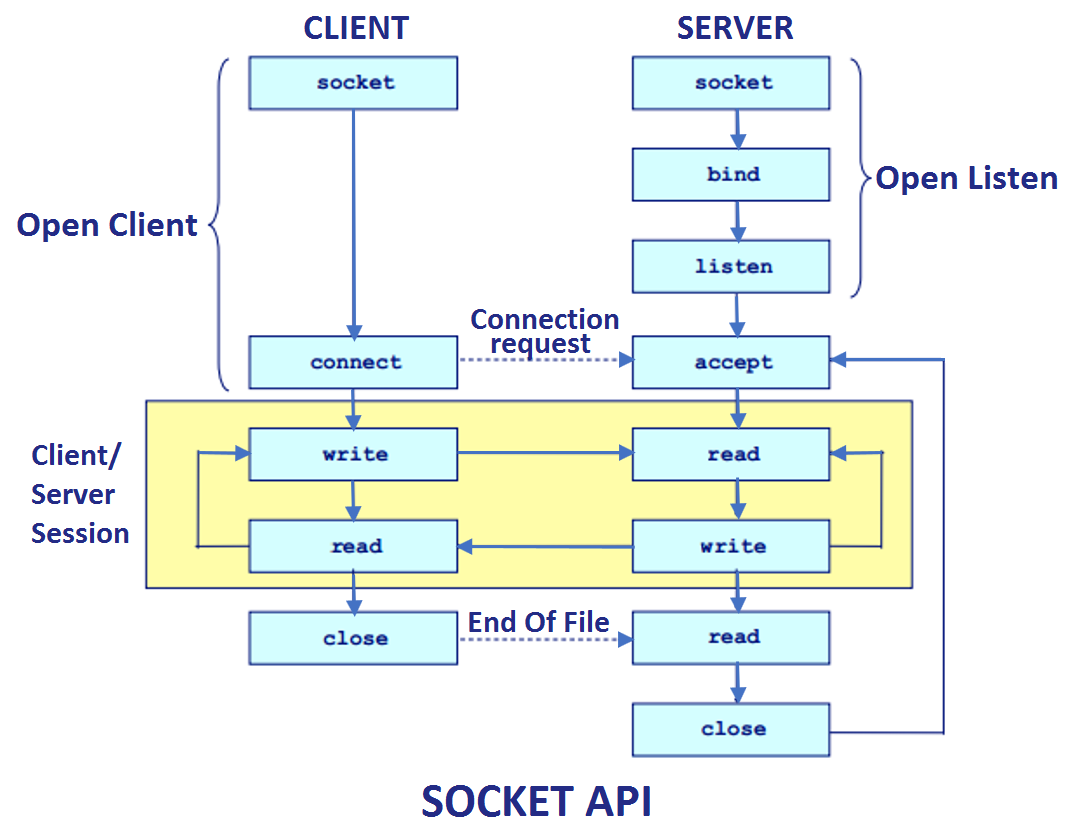
\includegraphics[width=.45\textwidth]{tcp-scheme.png}} 	\quad
    \subfloat[][\emph{TCP Header Format}]{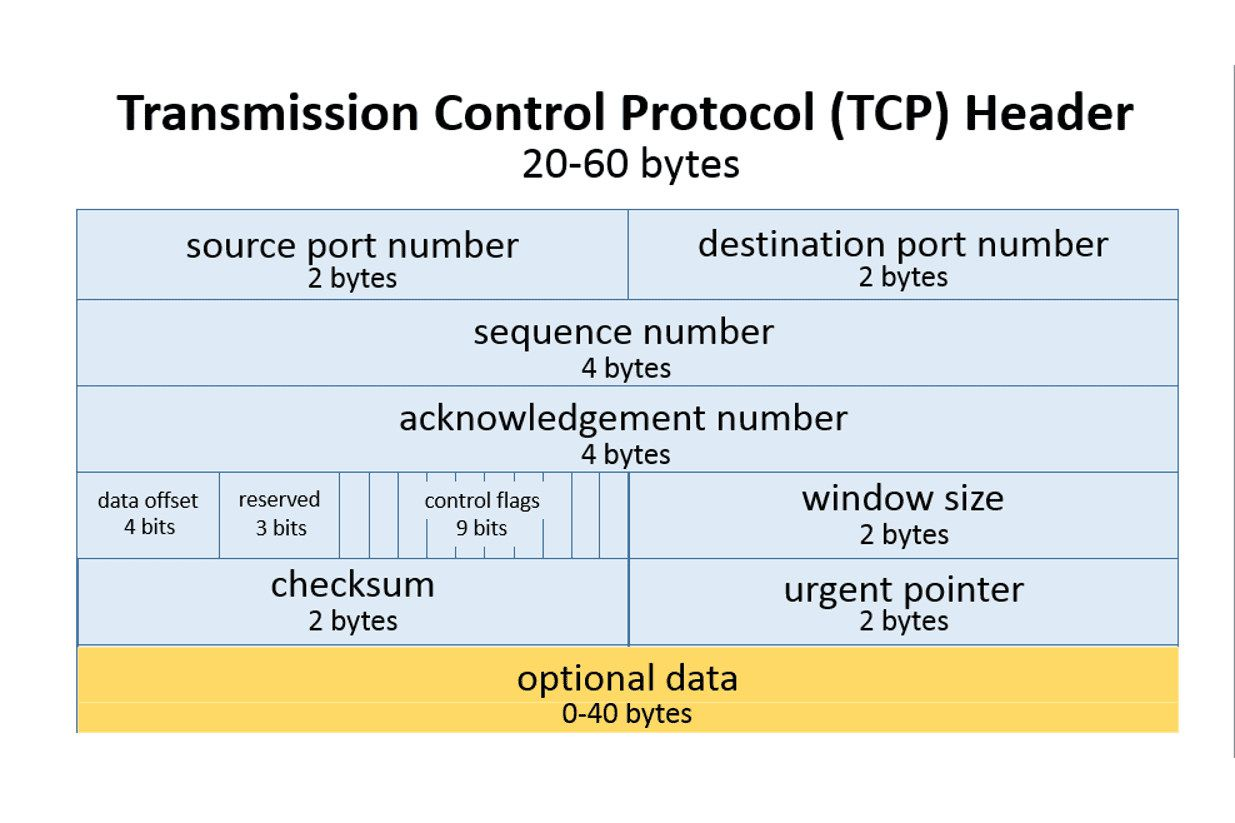
\includegraphics[width=.45\textwidth]{tcp-headers.jpg}}
    \captionsource{TCP protocol.}{%
    \href{https://www.lifewire.com/tcp-headers-and-udp-headers-explained-817970}{Lifewire}}
    \label{fig:tcp-scme}
\end{figure}
%
\subsection{Server implementation}
\label{ssec:soft-rasp-server}
In our case, it implements \texttt{QTcpSocket} network communication.  So, there
is a server service in main program shows in figure
(\ref{fig:software-socket-server}). While there is a client application deepened
later in section (\ref{sec:software-coral-intro}). Server application has
\texttt{QTcpSocket} and it listens to some port, in our case $52693$.
 Client has \texttt{QTcpSocket}, but has not connected to the server yet:\linebreak
%
%
\begin{figure}[!ht]
	\centering
	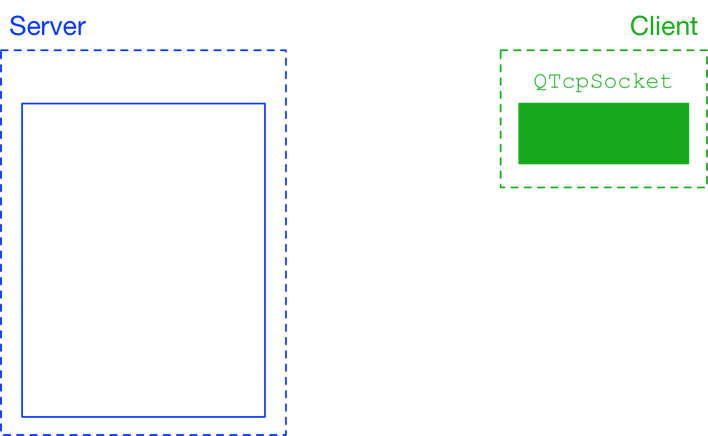
\includegraphics[width=0.7\textwidth]{qtcpserver-qtcpsocket.png}
	\caption{Interface client server \texttt{QTcpSocket}.}
	\label{fig:software-socket-server}
\end{figure}
%
\\When client connects to server, a \texttt{QTcpSocket} is created on the server’s
side, through which server and client can talk to each other and start send
message, shows in figure (\ref{fig:software-socket-server-client}).
%
%
\begin{figure}[htb]
	\centering
	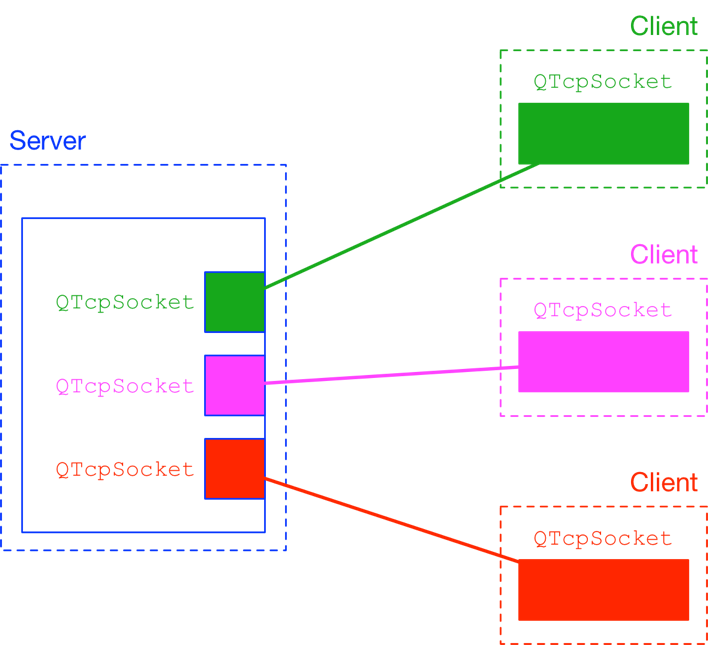
\includegraphics[width=0.55\textwidth]{qtcpserver-qtcpsocket-clients.png}
	\caption{Connection between server-clients.}
	\label{fig:software-socket-server-client}
\end{figure}
%
In particular, we observe the function reported in (\ref{lst:rasp-code-thread})
implemented in server application which sends the image just captured by the RGB
camera to the server to be  encapsulated in the message before send. 
In the function it is possible to observe the presence of a mutex which is 
locked to protect the resource and avoid overwriting through function calls.
The frame, i.e. the resource, is converted and stored in buffer before
sending.\\ 
Upon exiting the function body, the mutex is unlocked, thus giving free
access to resources again.
% code list
\begin{listing}[ht]
\inputminted[frame=lines,framesep=2mm, linenos=true, autogobble, breaklines=true, fontsize=\scriptsize, firstline=84, lastline=95]{c++}{software/code/mainwindow.cpp} 
\caption{Particular report function sending image.} 
\label{lst:rasp-code-thread} 
\end{listing}
